\section{การใช้งานแอปพลิเคชัน}
\subsection{การใช้งานหน้า Career Prediction}
ผู้ใช้สามารถเริ่มทำนายสายอาชีพได้จากการกดไปทำนายสายอาชีพ (1) ดังรูป \ref{fig:start-CP} ดังนี้
\begin{figure}[H]\centering
    \fbox{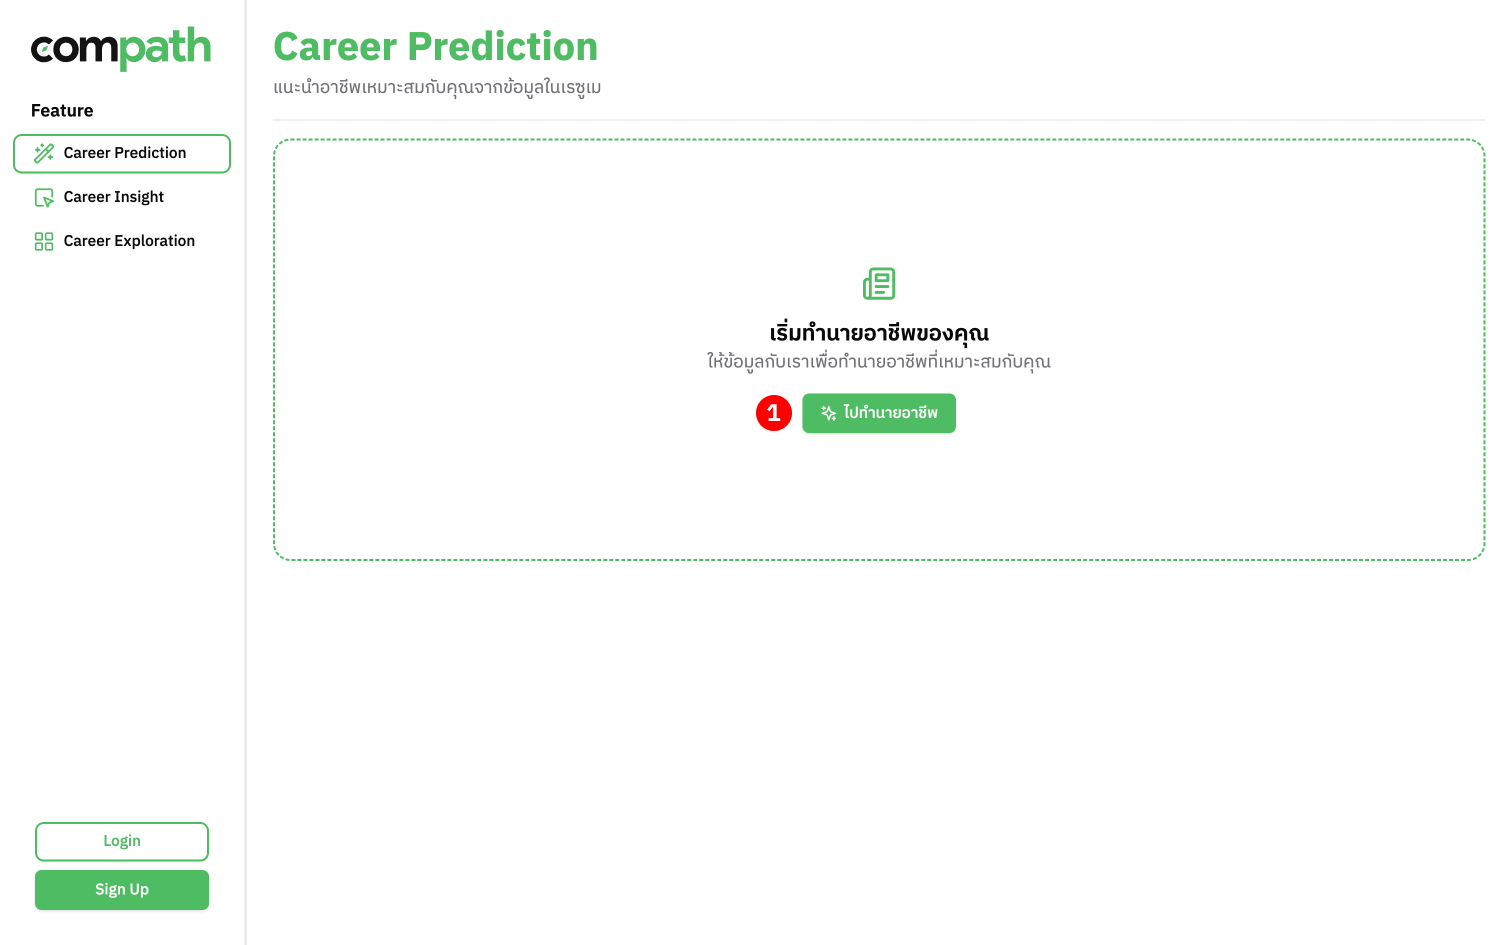
\includegraphics[width=13cm]{./figure/tutorial-picture/start-CP.png}}
    \caption{รูปแสดงหน้าหลักของหน้าทำนายสายอาชีพ}\label{fig:start-CP}
\end{figure}
จากนั้นผู้ใช้จะเริ่มการกรอกข้อมูลต่าง ๆ เพื่อนำข้อมูลไปใช้ในการทำนายสายอาชีพดังรูป \ref{fig:input-CP} ดังนี้
\begin{figure}[H]\centering
    \fbox{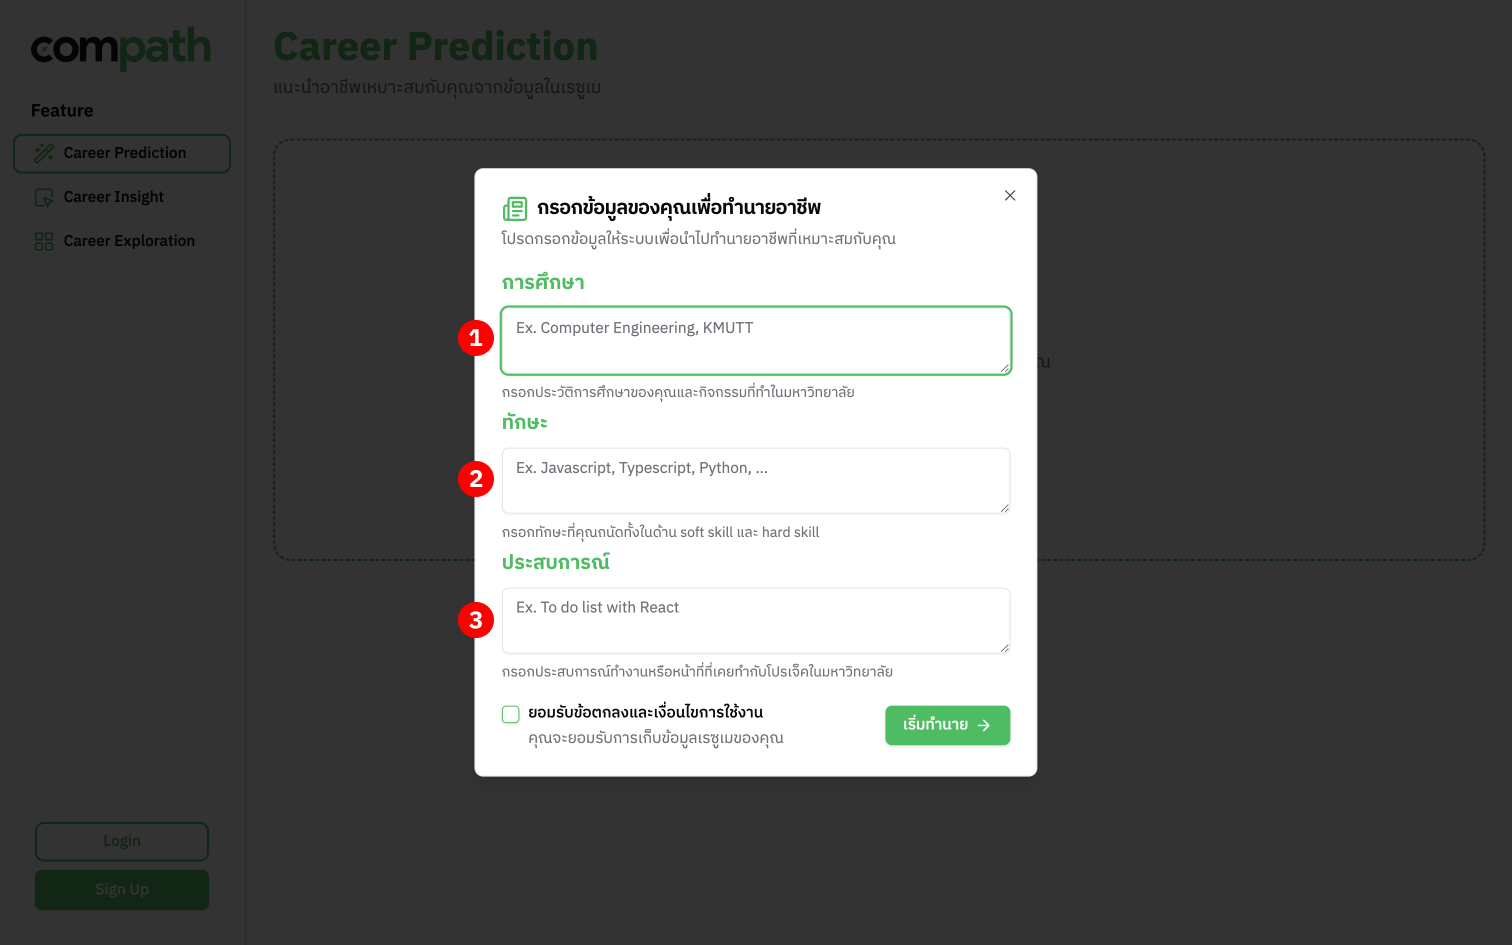
\includegraphics[width=13cm]{./figure/tutorial-picture/input-CP.png}}
    \caption{รูปแสดงการกรอกข้อมูลเพื่อทำนายสายอาชีพ}\label{fig:input-CP}
\end{figure}
ข้อมูลที่ผู้ใช้ต้องกรอกเพื่อทำนายสายอาชีพมีทั้งหมด 3 ส่วน ดังนี้

\begin{enumerate}
    \item \textbf{การศึกษา} คือ ประวัติการศึกษาและกิจกรรมที่เคยทำในมหาวิทยาลัยของผู้ใช้
    \item \textbf{ทักษะ} คือ ทักษะที่ผู้ใช้มีหรือถนัด
    \item \textbf{ประสบการณ์} คือ ประสบการณ์การทำงานหรือหน้าที่เคยรับผิดชอบในโปรเจ็คหรืองานในมหาวิทยาลัย
\end{enumerate}

โดยมีเงื่อนไขว่าผู้ใช้จำเป็นต้องกรอกให้ครบทั้ง 3 ส่วน จึงจะสามารถเริ่มการทำนายสายอาชีพได้ ถ้าหากกรอกไม่ครบระบบจะแสดงข้อความให้กรอกข้อมูลให้ครบดังรูป \ref{fig:warning-CP} ดังนี้
\begin{figure}[H]\centering
    \fbox{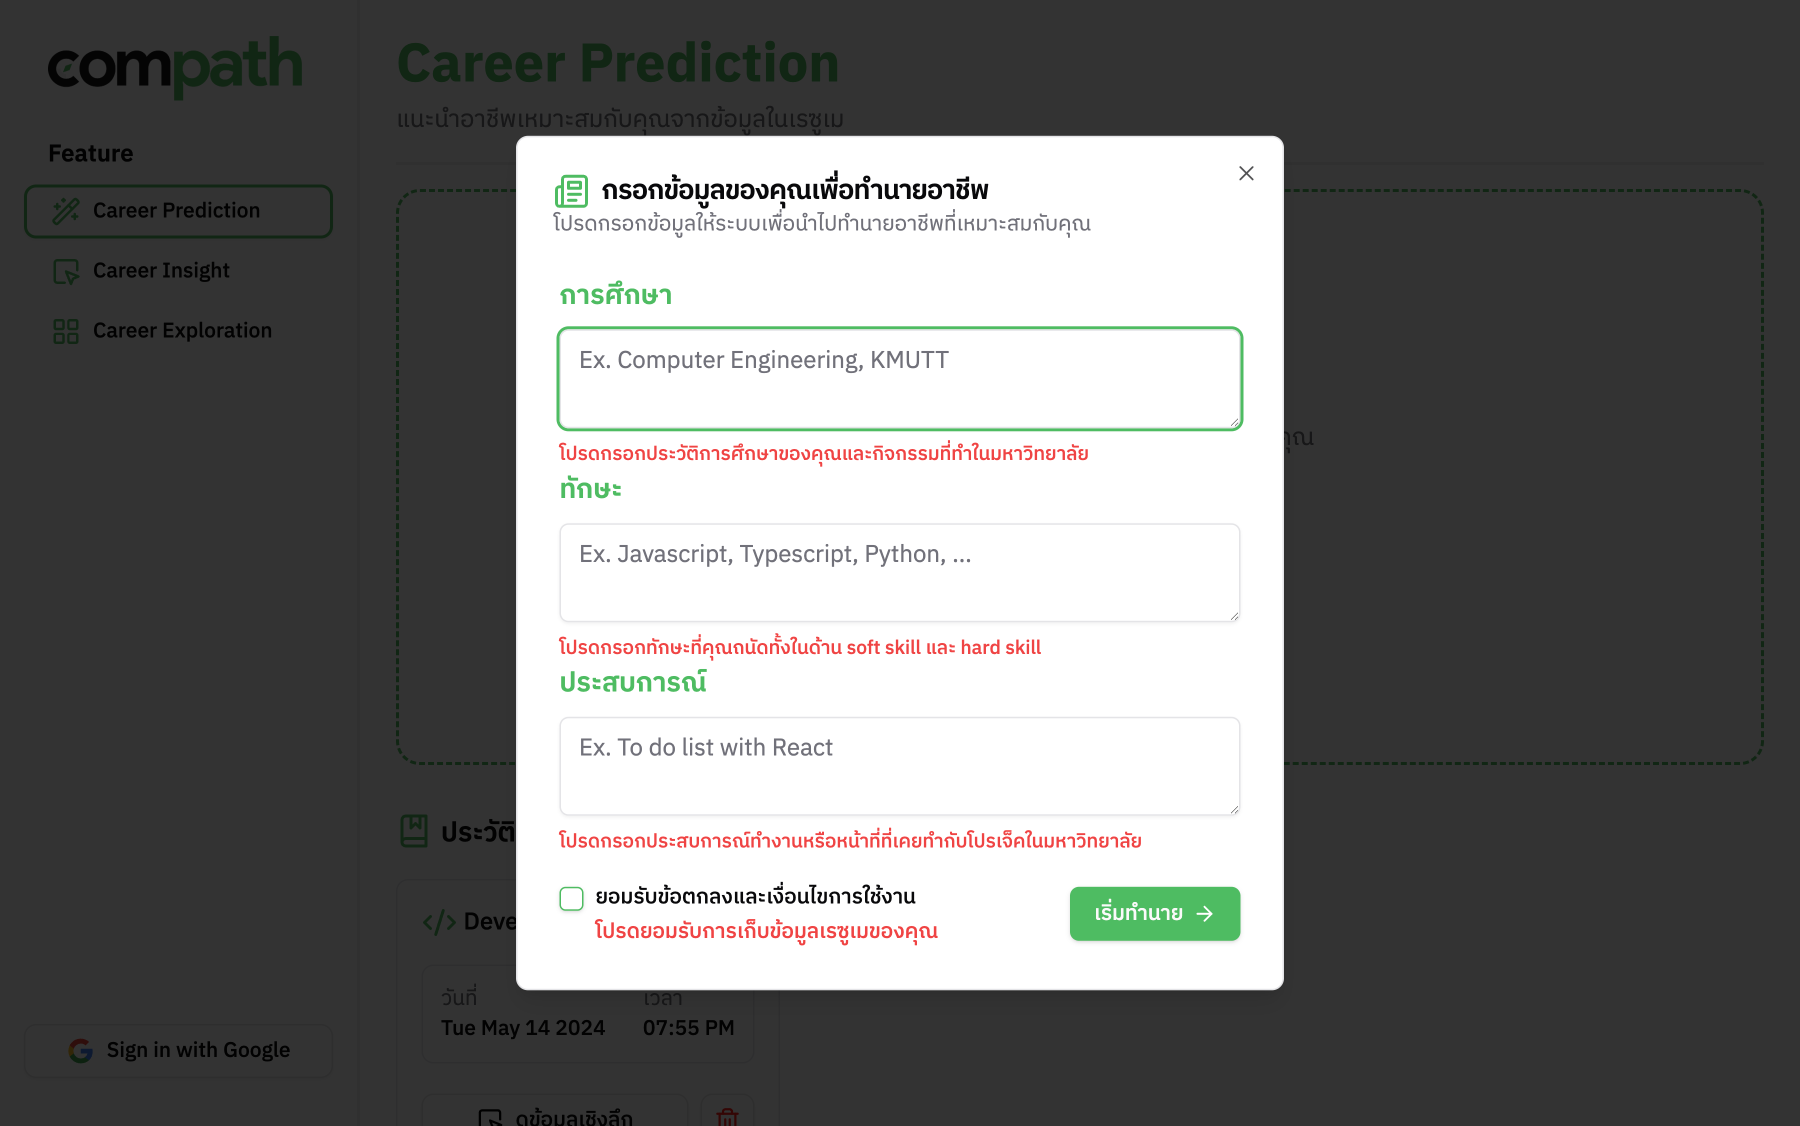
\includegraphics[width=13cm]{./figure/tutorial-picture/warning-CP.png}}
    \caption{รูปแสดงการแจ้งเตื่อนเมื่อผู้ใช้กรอกข้อมูลในการทำนายไม่ครบถ้วน}\label{fig:warning-CP}
\end{figure}
หลังจากผู้ใช้กรอกข้อมูลครบถ้วน ผู้ใช้จำเป็นต้องกดยอมรับข้อตกลงและเงื่อนไขการใช้งาน (1) เพื่อยินยอมการเก็บข้อมูลที่ผู้ใช้กรอก จึงจะสามารถเริ่มทำนายสายอาชีพได้ โดยจะเริ่มทำนายสายอาชีพเมื่อผู้ใช้กดเริ่มทำนาย (2) ดังรูป \ref{fig:accept-CP} ดังนี้
\begin{figure}[H]\centering
    \fbox{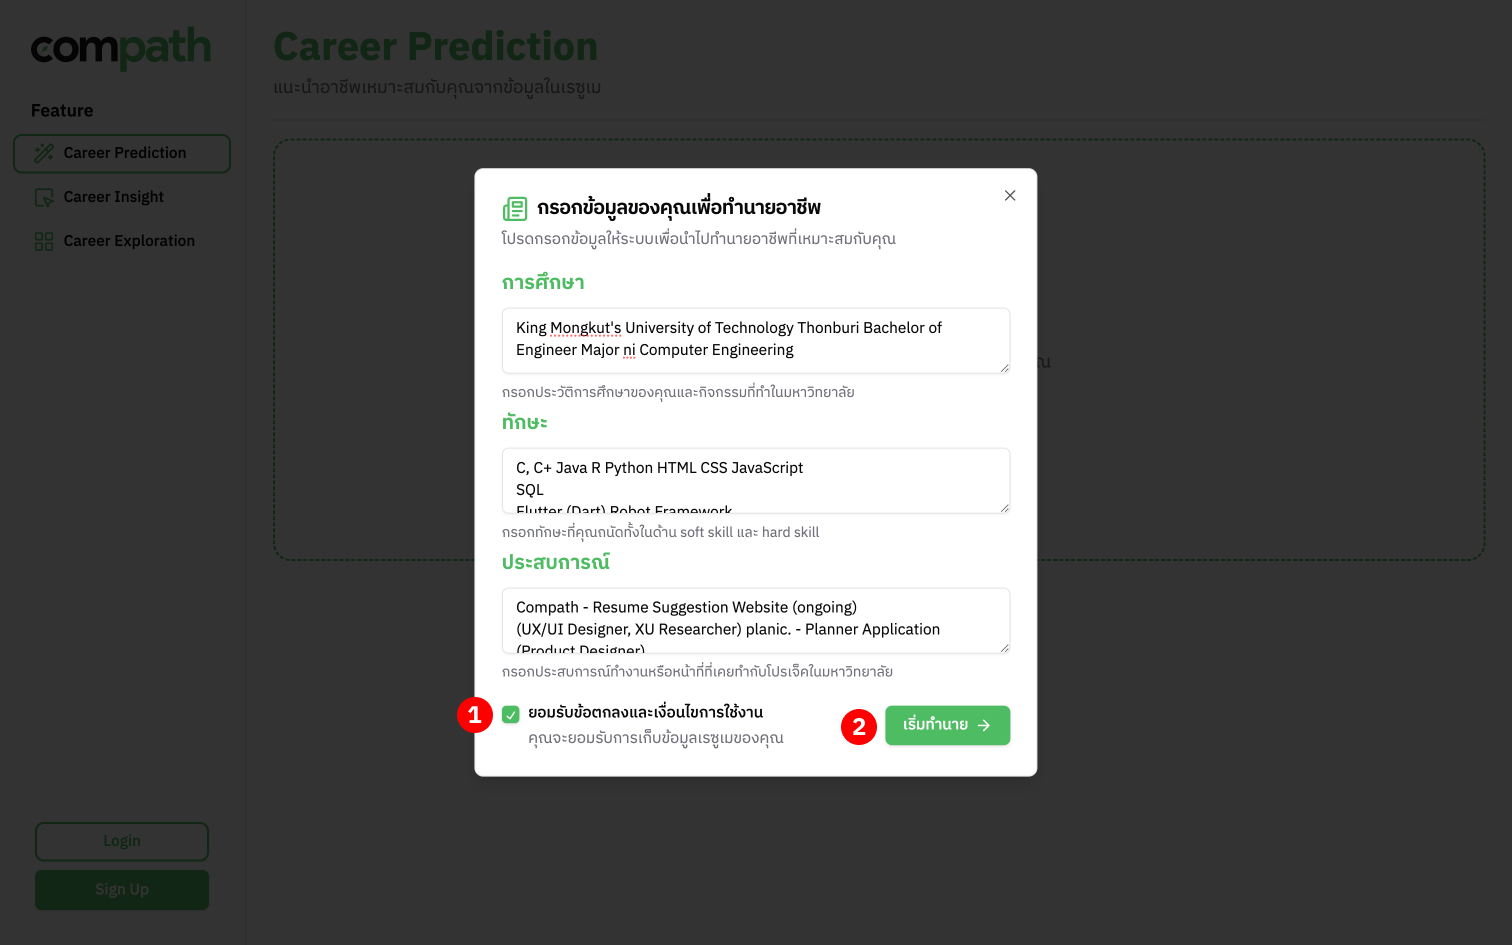
\includegraphics[width=13cm]{./figure/tutorial-picture/accept-CP.png}}
    \caption{รูปแสดงการยอมรับข้อตกลงการเก็บข้อมูลและเริ่มการทำนายสายอาชีพ}\label{fig:accept-CP}
\end{figure}
จากนั้นระบบจะแสดงอาชีพที่เหมาะสมโดยอ้างอิงจากข้อมูลที่ผู้ใช้กรอกมา และแสดงข้อมูลพื้นฐานของสายอาชีพที่ทำนายได้ รวมถึงผู้ใช้ยังสามารถดูข้อมูลเชิงลึกของสายอาชีพดังรูป ... ได้จาการกดดูเพิ่มเติม (1) และยังสามารถบันทึก (2) และแก้ไข (3) การทำนายสายอาชีพได้ดังรูป \ref{fig:viewmore-CP} ดังนี้
\begin{figure}[H]\centering
    \fbox{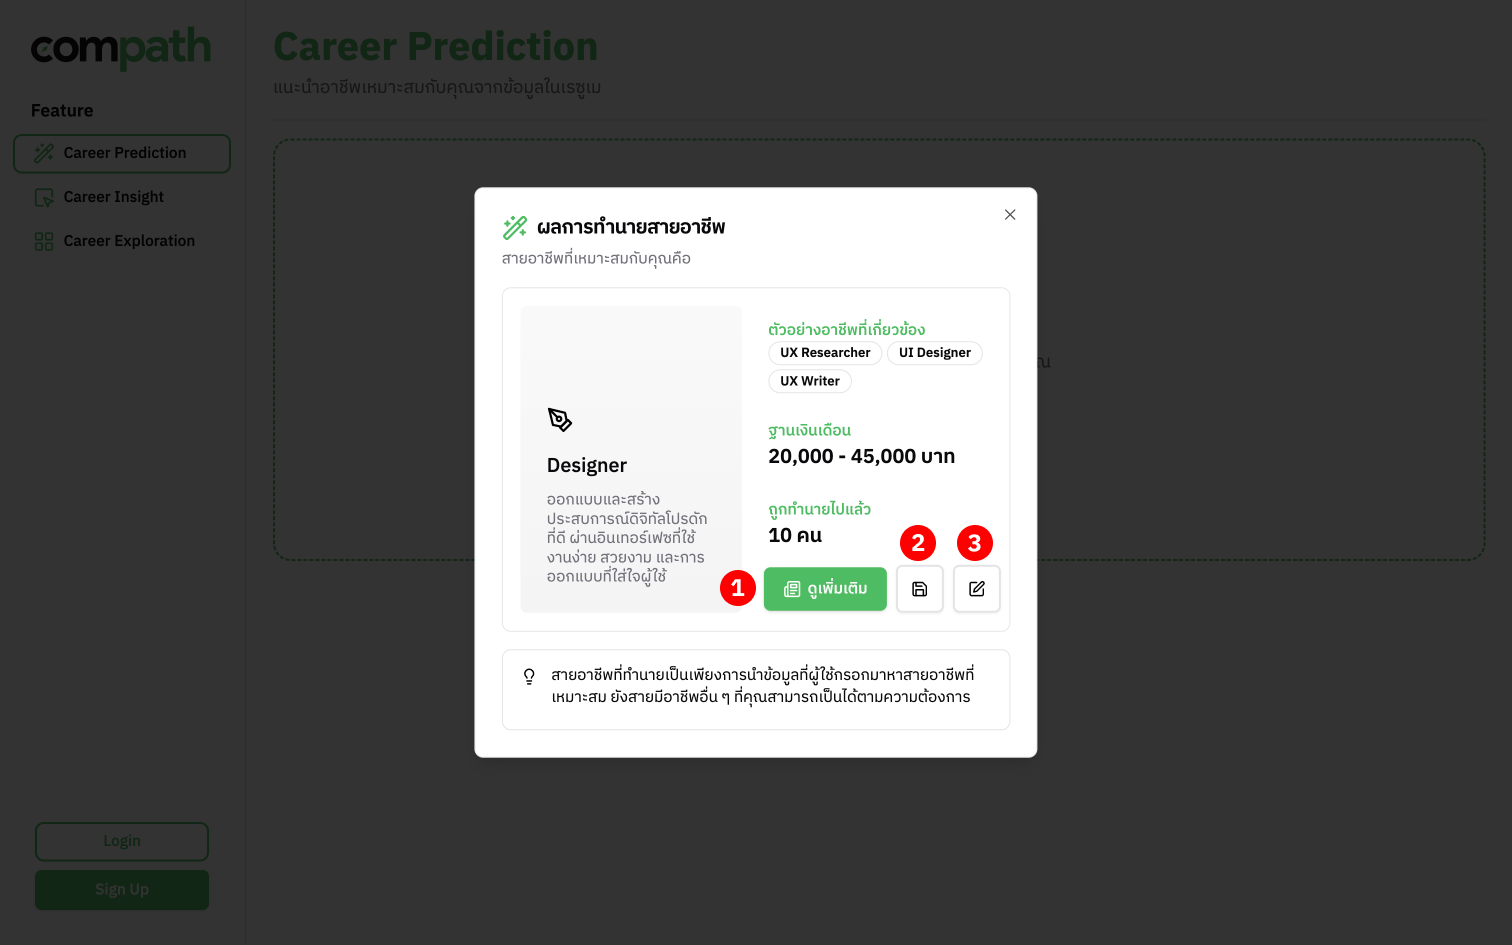
\includegraphics[width=13cm]{./figure/tutorial-picture/viewmore-CP.png}}
    \caption{รูปแสดงหน้าผลการทำนายสายอาชีพ}\label{fig:viewmore-CP}
\end{figure}
โดยเมื่อผู้ใช้บันทึกผลการทำนายสายอาชีพแล้วระบบจะแสดงการ์ดที่ทำนายไว้ เพื่อให้ผู้ใช้สามารถดูข้อมูลต่าง ๆ ที่เคยทำนายไว้ได้ รวมถึงสามารถเปิดเมนู (1) เพื่อแก้ไข (2) และลบ (3) การ์ดที่เคยทำนายสายอาชีพไว้ได้ดังรูป \ref{fig:cardhistory-CP} ดังนี้
\begin{figure}[H]\centering
    \fbox{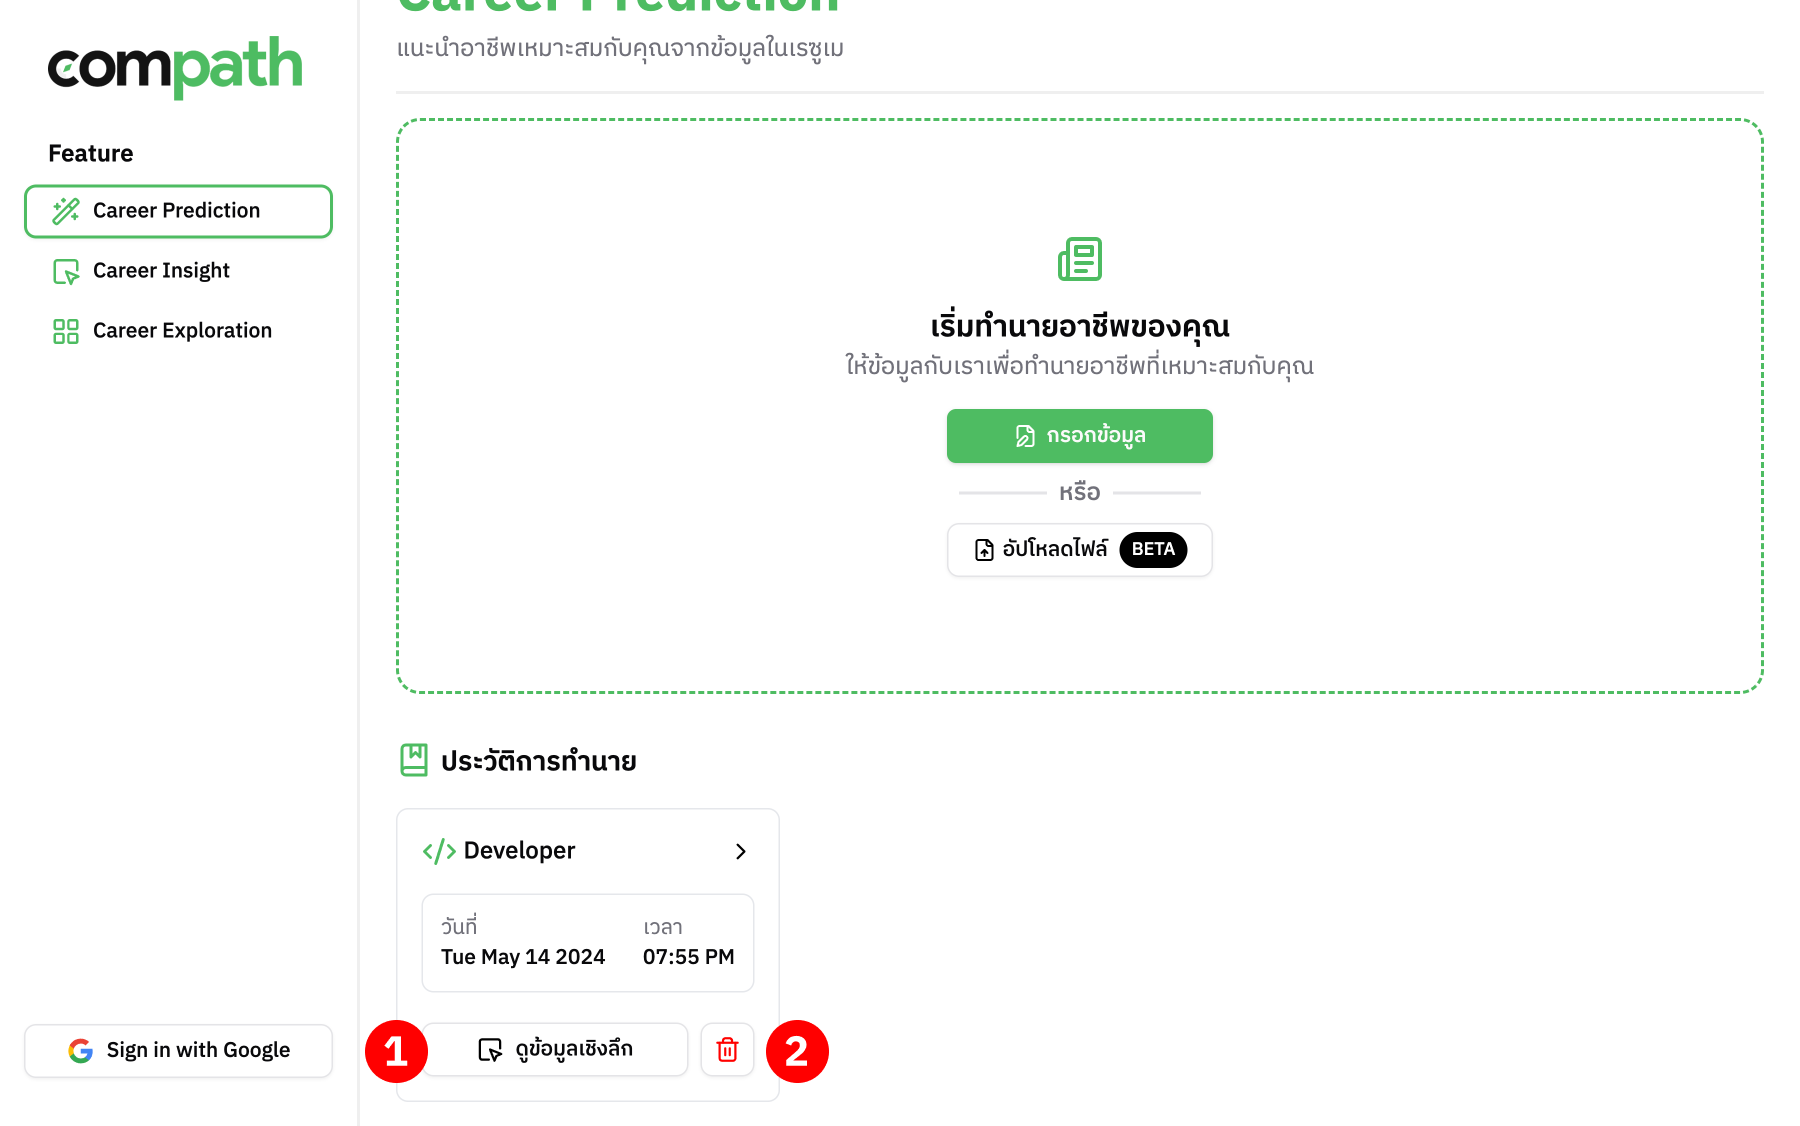
\includegraphics[width=13cm]{./figure/tutorial-picture/cardhistory-CP.png}}
    \caption{รูปแสดงหน้าหลักของหน้าทำนายสายอาชีพที่มีประวัติการทำนายแล้ว}\label{fig:cardhistory-CP}
\end{figure}
\subsection{การใช้งานหน้า Career Insight}
ผู้ใช้สามารถดูข้อมูลเชิงลึกของสายอาชีพที่ถูกทำนายได้ดังภาพ \ref{fig:home-CI} ดังนี้
\begin{figure}[H]\centering
    \fbox{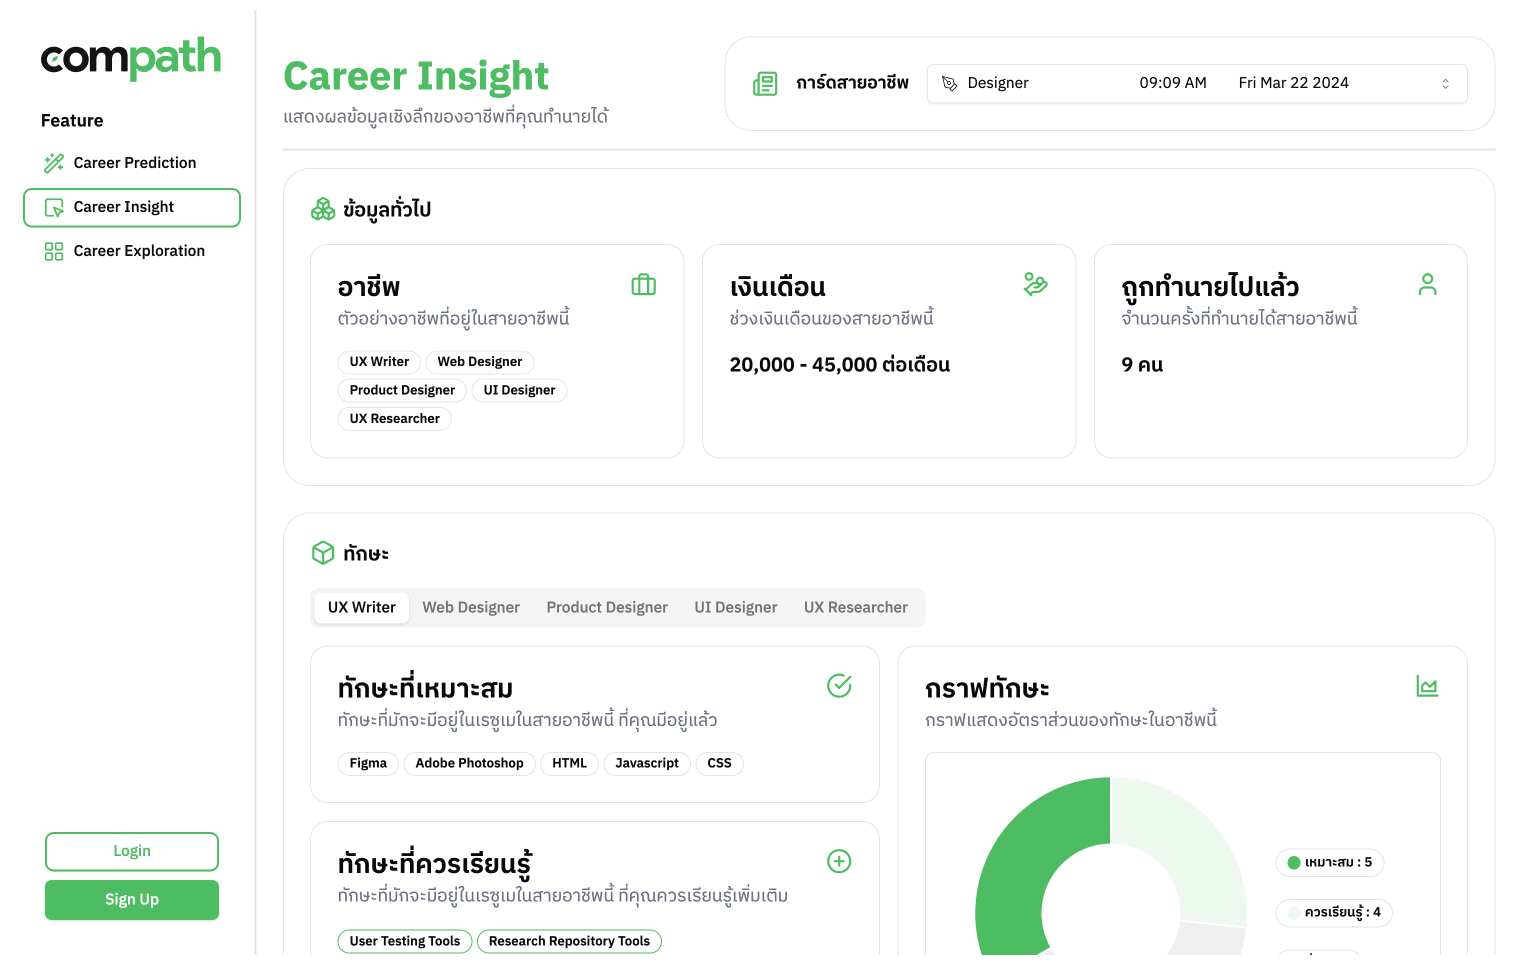
\includegraphics[width=13cm]{./figure/tutorial-picture/home-CI.png}}
    \caption{รูปแสดงการเข้าสู้หน้าหลักข้อมูลเชิงลึกของสายอาชีพ}\label{fig:home-CI}
\end{figure}
หลังจากเข้าสู้หน้าหลักของข้อมูลเชิงลึกแล้ว ผู้ใช้จะเห็นข้อมูลต่าง ๆ ของสายอาชีพที่ทำนายได้ โดยจะแบ่งออกเป็น 2 ส่วนหลัก ๆ ดังนี้ 
\begin{enumerate}
    \item \textbf{ข้อมูลทั่วไป} คือ ข้อมูลทั่วไปที่เกี่ยวกับสายอาชีพ โดยประกอบไปด้วย ตัวอย่างอาชีพที่อยู่ในสายอาชีพ ช่วงเงินเดือนของสายอาชีพ และจำนวนครั้งที่มีผู้ใช้ทำนายได้สายอาชีพนี้ ที่เหมือนกับข้อมูลที่แสดงในผลการทำนายดังรูป \ref{fig:viewmore-CP}
    \item \textbf{ทักษะ} คือ ทักษะที่เกี่ยวกับสายอาชีพที่ โดยแสดงให้ผู้ใช้เห็นเป็นลิสต์ของทักษะและกราฟอัตราส่วนของทักษะ ซึ่งจะแบ่งทักษะออกมาเป็น 3 ส่วน ดังนี้
    \begin{enumerate}
        \item \textbf{ทักษะที่เหมาะสม} คือ ทักษะที่ผู้ใช้กรอกมาจากฟังก์ชันการทำนายสายอาชีพดังรูป \ref{fig:accept-CP} และมักพบอยู่ในเรซูเมของอาชีพนี้
        \item \textbf{ทักษะที่ควรเรียนรู้} คือ ทักษะที่ควรเรียนรู้เพิมเติ่มเพื่อให้เรซูเมเหมาะสมกับอาชีพนี้มากขึ้น
        \item \textbf{ทักษะอื่น ๆ} คือ ทักษะที่ไม่เกี่ยวข้องกับอาชีพนี้โดยตรง แต่ผู้ใช้กรอกมาในฟังก์ชันการทำนายสายอาชีพดังรูป \ref{fig:accept-CP}
    \end{enumerate}
\end{enumerate}
\begin{figure}[H]\centering
    \fbox{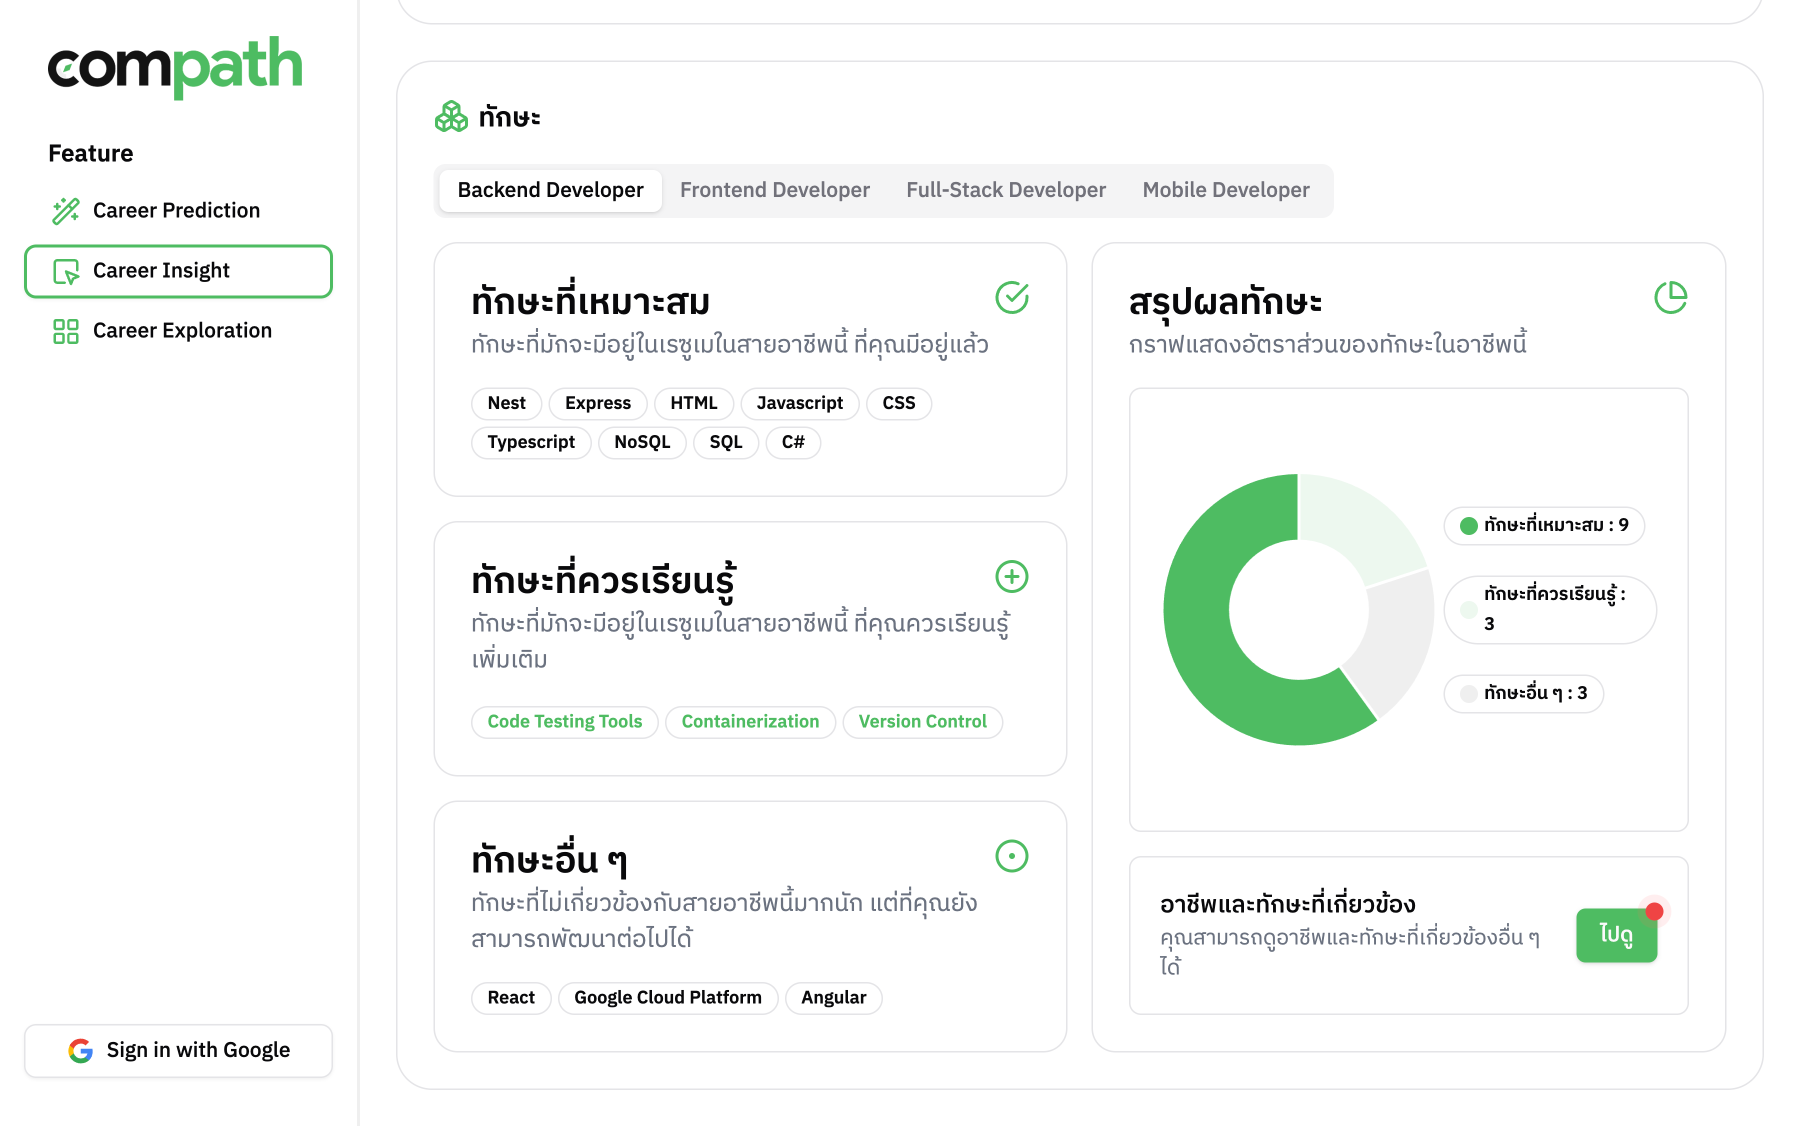
\includegraphics[width=13cm]{./figure/tutorial-picture/skillinfo-CI.png}}
    \caption{รูปแสดงส่วนทักษะในหน้าข้อมูลเชิงลึกของสายอาชีพ}\label{fig:skillinfo-CI}
\end{figure}
\begin{figure}[H]\centering
    \fbox{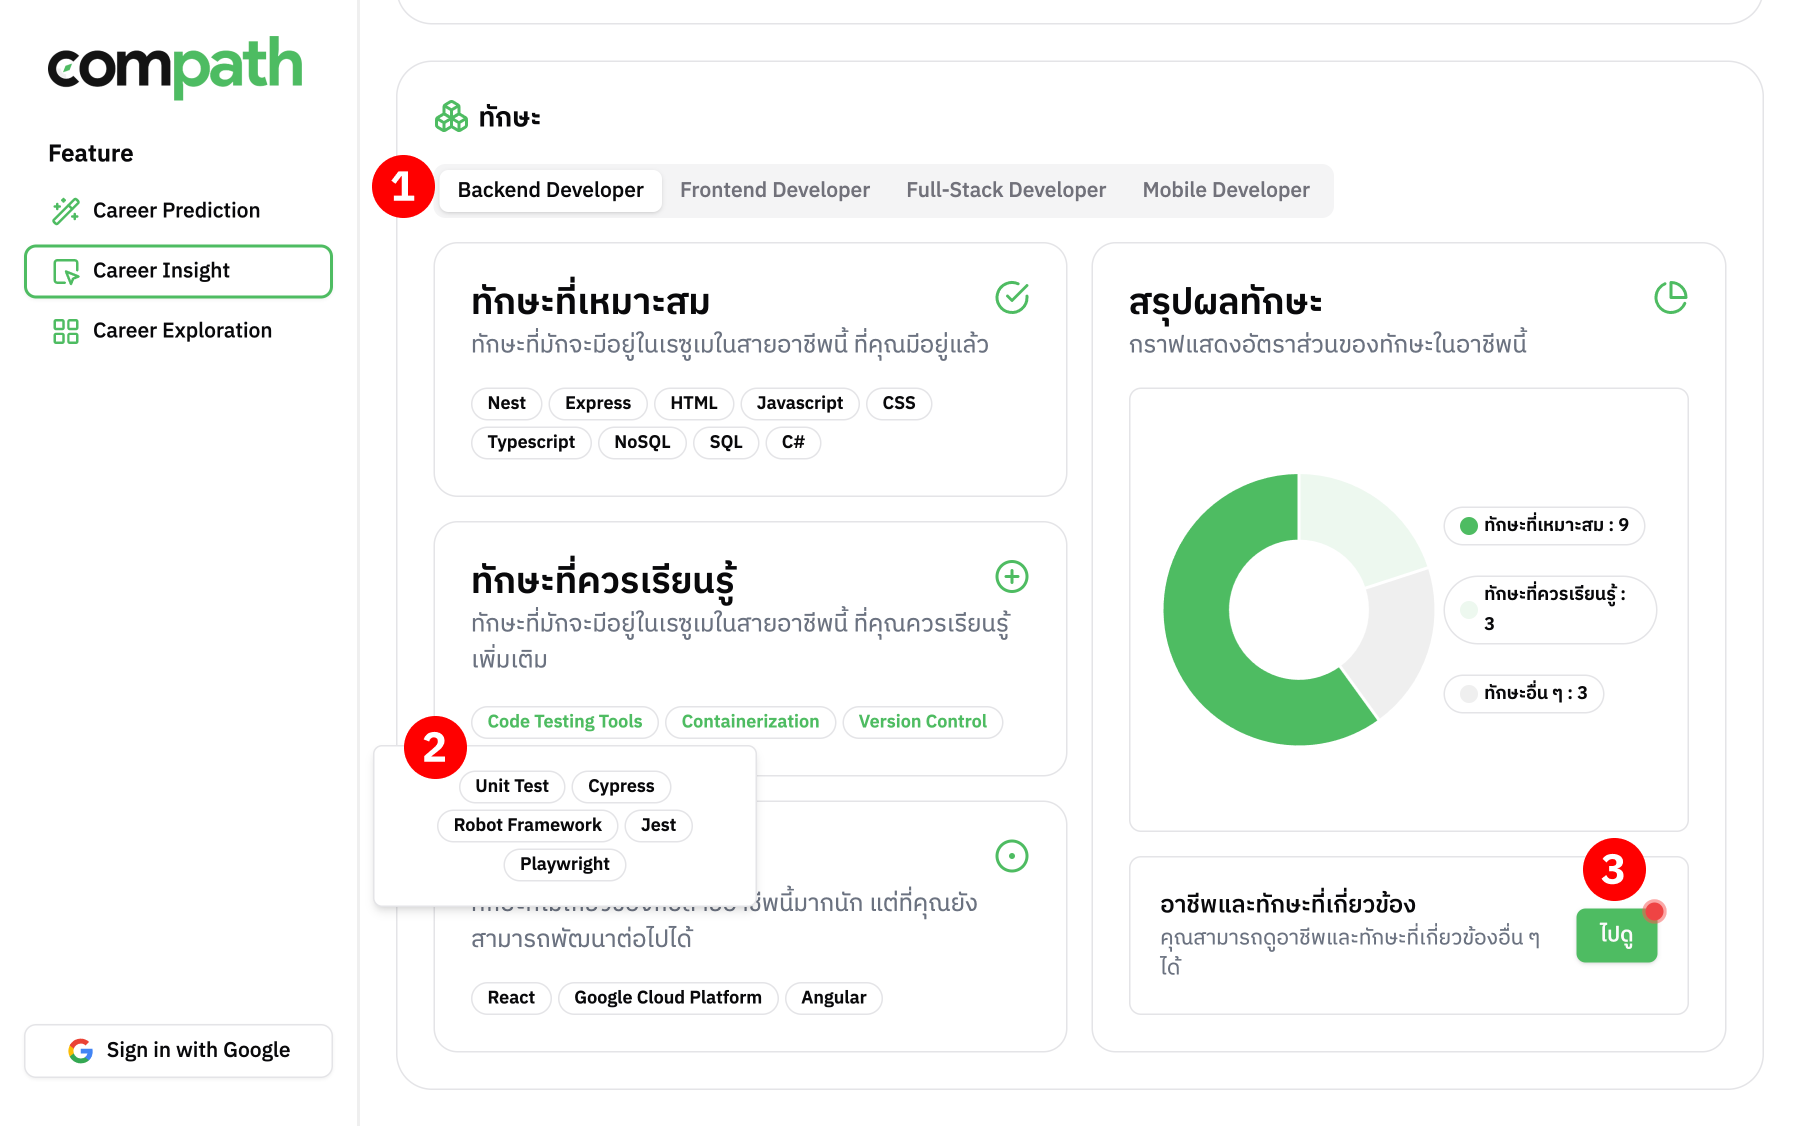
\includegraphics[width=13cm]{./figure/tutorial-picture/skillaction-CI.png}}
    \caption{รูปแสดงการใช้งานในส่วนทักษะ}\label{fig:skillaction-CI}
\end{figure}
\begin{figure}[H]\centering
    \fbox{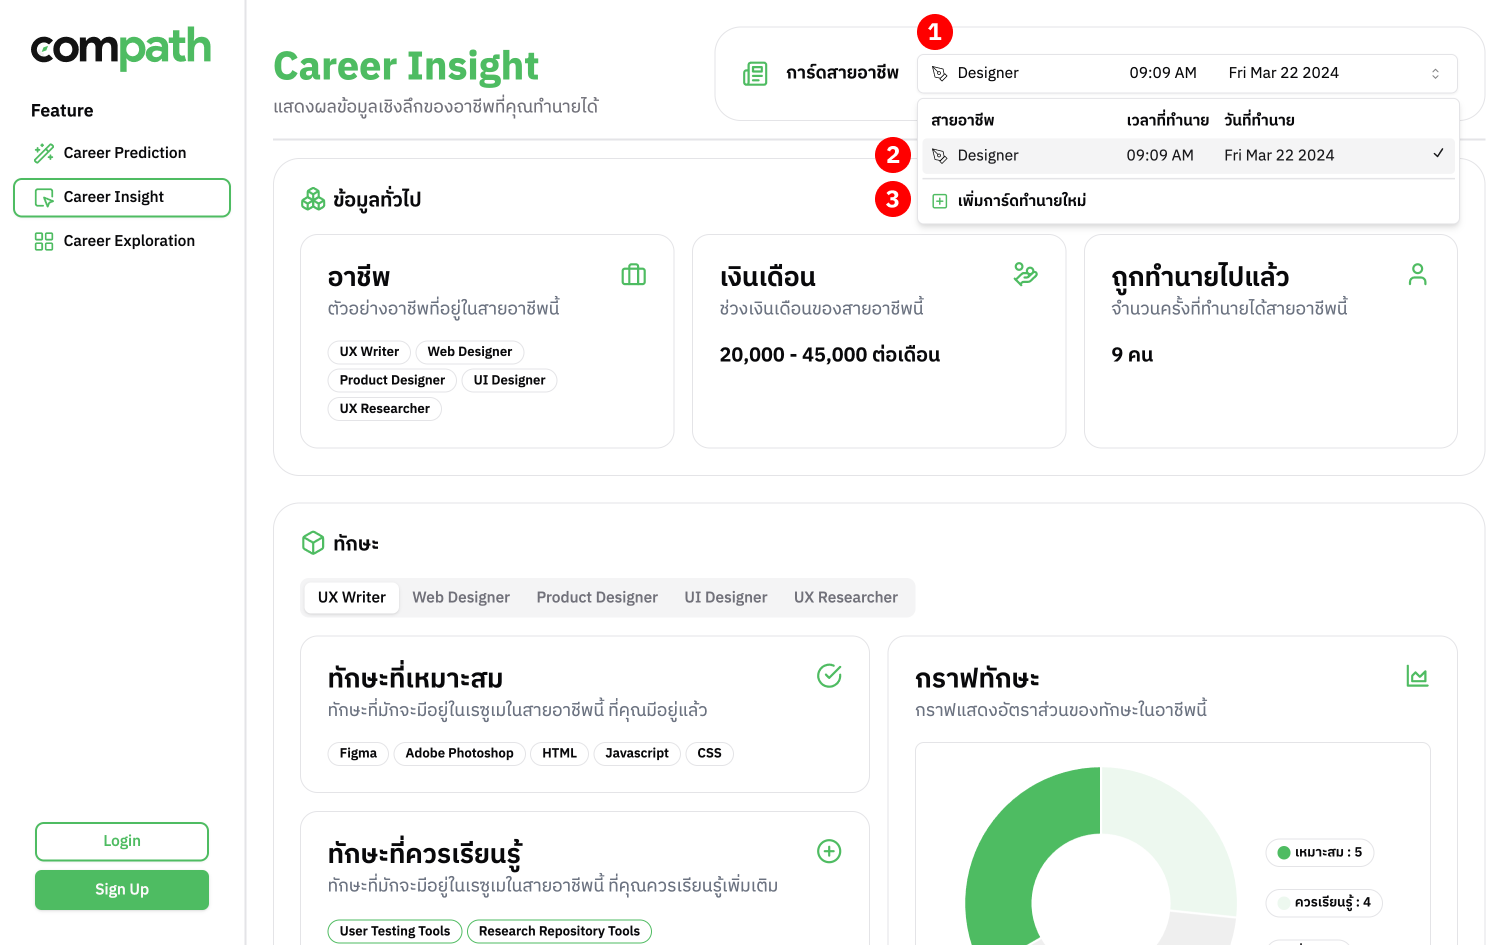
\includegraphics[width=13cm]{./figure/tutorial-picture/cardhistory-CI.png}}
    \caption{รูปแสดงการใช้งานเลือกการ์ดสายอาชีพเพื่อดูข้อมูลเชิงลึก}\label{fig:cardhistory-CI}
\end{figure}


\subsection{การใช้งานหน้า Career Exploration}
ผู้ใช้สามารถดูสายอาชีพต่าง ๆ ได้ดังภาพ \ref{fig:home-CE} ดังนี้
\begin{figure}[H]\centering
    \fbox{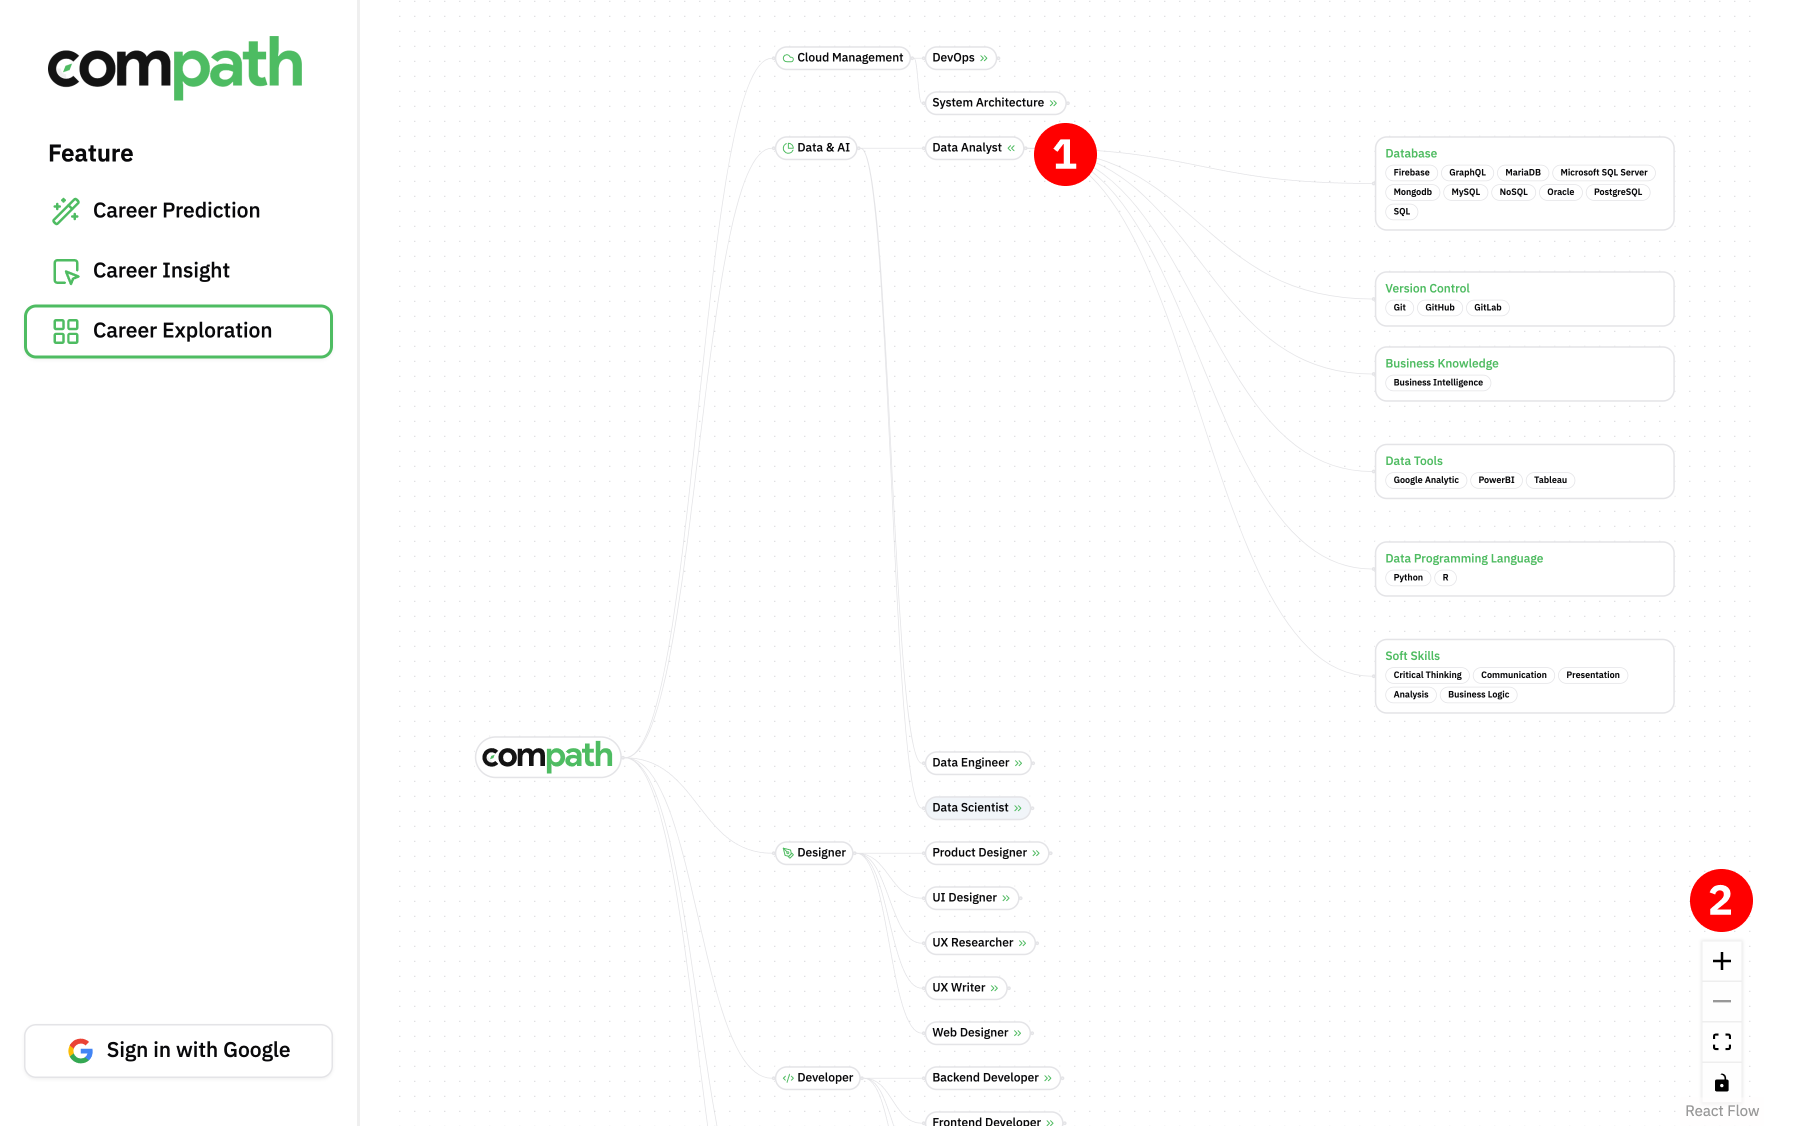
\includegraphics[width=13cm]{./figure/tutorial-picture/home-CE.png}}
    \caption{รูปแสดงการเริ่มทำนายสายอาชีพ}\label{fig:home-CE}
\end{figure}